\documentclass[10pt]{beamer}
\usepackage[T1]{fontenc}
\usepackage[utf8]{inputenc}
\usepackage[slovene]{babel}
\usepackage{pgfpages} % privat zapiski
\usepackage{amsmath} % pravilen izpis v "math mode"
\usepackage{hyperref}
\usepackage{pgfplots}
\usepackage{tikz}
%\documentclass{standalone}
%\usepackage{pgfplotstable,filecontents}
\usepackage[natbib=true,style=authoryear,backend=bibtex,useprefix=true]{biblatex}
\addbibresource{literatura_test}


\pgfplotsset{compat=1.8}
\hypersetup{hidelinks}
%\usetheme{Bergen}
\usecolortheme{seahorse}

\usepackage{graphicx}% http://ctan.org/pkg/graphicx
\usepackage{booktabs}% http://ctan.org/pkg/booktabs

\usepackage{palatino}
\usefonttheme{serif}

\setbeamertemplate{navigation symbols}{} % izklop navigacije
\setbeamertemplate{footline}[frame number]{} % oštevilčenje
\setbeamertemplate{note page}{\pagecolor{yellow!5}\insertnote}
\setbeamertemplate{itemize items}[circle]



\begin{document}
    \title[Diplomski seminar]{Iterativne numerične metode v posplošenih linearnih modelih}
    \author{Mitja Mandić \\ \small Mentor: izr. prof. dr. Jaka Smrekar}
    \date{1. april 2021} 

\begin{frame}
    \titlepage
\end{frame}


\begin{frame} \frametitle{Posplošeni linearni modeli}
    \begin{itemize}
    
        \item Slučajni del, sistematični del, povezovalna funkcija
        \pause
        \item Linearna regresija: 
            $$ \mathbb{E}(Y) = x ^ T\beta $$
        \item Problem - ni najboljša. Rešitev? Transformacija pričakovane vrednosti
    \end{itemize}
\end{frame}

\begin{frame} \frametitle{Logistični model}
    \begin{itemize}
    \item Za kategorične podatke $\rightarrow$ binomska porazdelitev
    \pause
    \item $ \mathrm{logit}(p_{i}) = \mathrm{log} (\frac{p_{i}}{1 - p_{i}}) = x ^ T\beta $ %\rightarrow p_{i} = \frac{ e^{x^T\beta}}{1 + e^{x^T\beta}} $
    \end{itemize}
\end{frame}

\begin{frame}

$$p = \frac{e^{x^T\beta}}{1+e^{x^T\beta}}$$
\begin{figure}   % treba še naštudirat da bo graf prou
    \begin{center}
        \begin{tikzpicture}

            \begin{axis}%
            [
                grid=major,     
                xmin=-10,
                xmax=10,
                axis x line=bottom,
                ytick={0,.5,1},
                ymax=1,
                axis y line=middle,
            ]
                \addplot%
                [
                    blue,%
                    mark=none,
                    samples=100,
                    domain=-6:6,
                ]
                (x,{1/(1+exp(-x))});
            \end{axis}
        \end{tikzpicture}

    \end{center}
\end{figure}
\end{frame}

\begin{frame} \frametitle{Točkovno ocenjevanje}
    \begin{itemize}
        \item \textit{Cenilka} je funkcija vzorca, s katero ocenjujemo določeno karakteristiko
        \pause
        \item Dve glavni metodi za določanje: metoda momentov in metoda največjega verjetja
    \end{itemize}
\end{frame}
\begin{frame} \frametitle{Metoda momentov}
    \begin{itemize}
        \item Enostavnejša za računanje brez računalnika
        \pause
        \item Karakteristiko izrazimo kot funkcijo momentov $c(X) = g(m_{1}(X), m_{2}(X),\ldots,m_{r}(X))$ in jo ocenimo z $g(\hat{m}_{1},\ldots,\hat{m}_{r})$
    \end{itemize}
\end{frame}

\begin{frame}{Metoda največjega verjetja}
    \begin{itemize}
        \item Najprej privzemimo gostote oblike $f_{X}(x;\theta) = f(x;\theta_{1},\ldots,\theta_{r})$ za nek $\theta \in \Theta$
        
        \item Pri fiksni realizaciji poskusa definiramo \textit{funkcijo verjetja}
        \[ \ell(X_{1},\ldots,X_{n};\underbrace{\theta_{1},\ldots,\theta_{r}}_{\theta}) = f(X_{1},\theta)\cdots f(X_{n},\theta) \]
        \item Iščemo $\theta,$ kjer bo imela maksimum, kar bo natanko ničla odvoda $\log \ell$
        \item Sistemu 
        \[
            \frac{\partial}{\partial \theta_{j}}\log \ell (X,\theta) = 0
        \]
        pravimo sistem enačb verjetja, njegova rešitev je \textit{cenilka največjega verjetja}
        \item Niso nujno nepristranske, so pa dosledne, če je rešitev enolična
        \item Običajno niso eksplicitno rešljive
    \end{itemize}
\end{frame}


\begin{frame} \frametitle{Eksponentna družina}
    \[
        f_{Y}(y; \theta, \phi) = \exp{\left(\frac{(y\theta - b(\theta))}{a(\phi)} + c(y, \phi)\right)}
    \]
    za neke $a(\cdot), b(\cdot)\text{~in~}c(\cdot).~\theta$ imenujemo tudi naravni parameter.
    
\end{frame}

\begin{frame}{Eksponentna družina}
Iz predavanj STAT1 se spomnimo, da velja
\[
    \mathbb{E}(\nabla \ell) = 0.
\]
Na podoben način z uporabo $\int f_{Y}(y;\theta) \,dy = 1$ pa dokažemo tudi \textit{informacijsko enakost}
\[
    \mathbb{E}(\frac{\partial^2}{\partial \theta^2}\ell(\theta)) = -\mathbb{E(\frac{\partial}{\partial \theta} \ell(\theta))^2}
\]
\end{frame}

\begin{frame}
    Z uporabo prve enakosti sledi
    \[
        \frac{\partial}{\partial \theta}\ell = \frac{y - b'(\theta)}{a(\phi)} \rightarrow \mu = b'(\theta)a(\phi)
    \]
    Iz druge pa:
    \begin{align*}
    %    
        \mathbb{E}(\frac{\partial^2}{\partial \theta^2}\ell) &= \mathbb{E}(\frac{b''(\theta)}{a(\phi)}) = \frac{b''(\theta)}{a(\phi)} \\
        \mathbb{E}((\frac{\partial}{\partial \theta} \ell)^{2}) &= \frac{1}{a(\phi)^2}\mathbb{E}((y-\mu)^2) = \frac{Var(Y)}{a(\phi)^2} 
    %
    \end{align*}
    od koder direktno sledi
    \[
        Var(Y) = -b''(\theta)a(\phi)
    \]
\end{frame}

\begin{frame}{Zgled z binomsko porazdelitvijo}
    Naj bo $Y \sim \mathrm{Bin}(n,p)$ Verjetnost 
    \[
        \mathrm{P}(Y = y) = \binom{n}{y}p^y(1-p)^{n-y} = \exp\left(y\log(\frac{p}{1-p}) + n\log(1-p) + \log{\binom{n}{k}}\right),
    \]
    od koder direktno sledi
    \[
        \theta = \log\frac{p}{1-p} = \log \frac{\mu}{1-\mu},~b(\theta) = \log(1 + e^{\theta}),~\phi = 1, a(\phi) = \frac{\phi}{n},
    \]
    V tem primeru velja torej $\theta = \textrm{logit}(\mu) = X^\top\beta = \eta$ in \textit{logit} je kanonična povezovalna funkcija za logistični model.
    Zakaj je to koristno?
\end{frame}
\begin{frame}\frametitle{Obvoz v numerične metode}

%\begin{frame}\frametitle{Numerične metode}
    \begin{itemize}
        \item Za ocenjevanje parametrov $\beta$ običajno rešujemo sistem enačb največjega verjetja
        \item v splošnem ni eksplicitno rešljiv in zato potrebujemo numerične metode
        \pause
        \item Newtonova metoda še vedno zelo aktualna zaradi kvadratična konvergence:
        $$x_{i+1} = x_{i} - \frac{f(x_{i})}{f'(x_{i})} $$
        Je pa to metoda za iskanje ničel in ne ekstremov!
    \end{itemize}
\end{frame}


\begin{frame}{Prilagoditev Newtonove metode}
    Najprej zapišimo Taylorjev polinom okoli iskane vrednosti $\theta$
    \[
        L(\theta) \approx L(\theta_{n}) + dL(\theta_{n})(\theta - \theta_{n}) + \frac{1}{2}(\theta - \theta_{n})^\top d^{2}L(\theta_{n})(\theta - \theta_{n})
    \]
    \pause
    Iščemo ekstrem funkcije torej ničlo odvoda in zato
    \[
        \ell(\theta*) = 0 \approx \ell(\theta_{0})(\theta*-\theta_{0})
    \]
    Izrazimo in dobimo iteracijski korak
    \[
        \theta_{t} = \theta_{t-1}-\frac{\ell(\theta_{t-1})}{\ell'(\theta_{t-1})}
    \]
    \pause
    Kaj gre lahko narobe?
\end{frame}

\begin{frame}{Prilagoditev Newtonove metode}
    \begin{itemize}
        \item Invertiranju Hessiana se lahko izognemo z uporabo premikov:
        \[
            \theta_{t} = \theta_{t-1} + h_{t-1}
            \ell'(\theta_{t-1})h_{t-1} = -\ell(\theta_{t-1})
        \]
        \pause
        \item Newtonova metoda ni naraščajoč algoritem $\Rightarrow$ ne vemo ali se bo premikal navzgor ali navzdol
        \pause
        \item Če je Hessejeva matrika pozitivno definitna je algoritem konstanten!
    \end{itemize}
\end{frame}

\begin{frame}{Fisher scoring}
    \[
        \beta_{i+1} = \beta_{i} + \frac{\dot{l}(\beta_{i})}{E(\ddot{l}(\beta_{i}))} 
    \]
    \pause
    Nazaj k eksponentni družini:
    \[
        \log f_{y}(y;\theta) = L(y;\theta) = \frac{y\theta-b(\theta)}{a(\phi)}
    \]
\end{frame}

\begin{frame}
    \[
    \frac{\partial L}{\partial\beta_{j}} = (\frac{\partial L}{\partial \theta})(\frac{\partial \theta}{\partial\mu})(\frac{\partial\mu}{\partial\eta})(\frac{\partial\eta}{\partial\beta_{j}})
    \]
    \begin{itemize}
        \item $\frac{\partial L}{\partial \theta} = \frac{y-b'(\theta)}{a(\phi)}$
        \pause
        \item Z uporabo $(b')^{-1}(\mu) = \theta$ dobimo $\frac{\partial \theta}{\partial\mu} = \frac{1}{b''(\theta)} = \frac{a(\phi)}{var(Y)}$
        \pause
        \item $(\frac{\partial \mu}{\partial \eta})$ bo odvisen od povezovalne funkcije, s tem se bomo ukvarjali pozneje
        \pause
        \item $(\frac{\partial \eta}{\partial\beta_{j}}) = x_{ij}$
    \end{itemize}
    \pause
    Končno,
    \[
        \frac{\partial L}{\partial\beta_{j}} = \frac{y-\mu}{var(Y)}\frac{\partial \mu}{\partial\eta}x_{ij}
    \]
\end{frame}


\begin{frame}{Ujemanje F-S in N-R}
    Če pa uprabimo kanonično povezovalno funkcijo je $\theta = \eta$ in zato $\frac{\partial \mu}{\partial \theta} = b''(\theta)$ in funkcija zbira postane
    \[
        \frac{\partial L}{\partial\beta_{j}} = \frac{y-\mu}{var(Y)}b''(\theta)x_{ij} = \frac{y-\mu}{a(\phi)}x_{ij}
    \]
    \pause
    Uporabimo $\mathrm{E}(\frac{\partial^2 L}{\partial\theta^2}) = -\mathrm{E}((\frac{\partial L}{\partial\theta})^2):$
    \begin{align*}
        -\mathbf{E}(\frac{\partial^2 L}{\partial\beta_{j}\partial\beta_{k}}) &= \mathbf{E}((\frac{\partial L}{\partial \beta_{j}})(\frac{\partial L}{\partial \beta_{k}})) \\
        &= \mathbf{E}(\frac{y-\mu}{var(Y)^2})(\frac{\partial\eta}{\partial\mu})^{2}x_{ij}x_{ik} \\
        &= \frac{1}{var(Y)}(\frac{\partial\eta}{\partial\mu})^{2}x_{ij}x_{ik} \\
        &= \frac{b''(\theta)}{a(\phi)}x_{ij}x_{ik}
    \end{align*}

\end{frame}

\begin{frame}
    Po drugi strani pa je odvod funkcije zbira
    \begin{align*}    
        \frac{\partial^2L}{\partial\beta_{j}\partial\beta_{k}} &= \frac{\partial}{\beta_{k}}\{\left(\frac{\partial L}{\partial\theta}\right)\left(\frac{\partial \theta}{\partial\beta_{j}}\right)\}\\
        &= \frac{\partial\L}{\partial\theta}\left(\frac{\partial^2\theta}{\partial\beta_{j}\partial\beta_{k}}\right) + \left(\frac{\partial\theta}{\partial\beta_{j}}\right)\left(\frac{\partial^2L}{\partial\theta^2}\frac{\partial\theta}{\partial\beta_{k}}\right) \\
        &= 0 + \frac{\partial^2L}{\partial\theta^2}x_{ij}x_{ik},
    \end{align*}
    videli pa smo že da je
    \[
        \frac{\partial^2L}{\partial\theta^2} = -\frac{b''(\theta)}{a(\phi)}.
    \]
    Sledi torej, da za kanonično povezovalno funkcijo Fisher-scoring in Newton Raphson sovpadata!
\end{frame}
\begin{frame}
    Še več, iz predavanj se spomnimo da je
    \[
        FI(\theta) = var(\frac{\partial}{\partial \theta}L)
    \]
    ==> Hessejeva matrika je za kanonično povezovalno funkcijo pozitivno definitna in Fisher scoring metoda je naraščajoča!
\end{frame}

\begin{frame} \frametitle{Enačbe verjetja v logističnem modelu}
    Imejmo slučajni vektor $Y = (Y_{1}, \ldots, Y_{n})$ z NEP komponentami porazdeljenimi binomsko 
    \[
        P(Y_{i} = y_{i}) = {n_{i} \choose y_{i}} p_{i}^{y_{i}}(1 - p_{i}) ^{m_{i} - y_{i}}
    \]
    Funkcija verjetja se glasi:
    \begin{align*} %preveri spacing med vrsticami
        \ell(p_{i}) &= \log\{\prod_{i=1}^{n} p_{i}^{y_{i}}(1 - p_{i})^{m_{i} - y_{i}} \}  \\
            &= \sum_{i=1}^{n}\{y_{i}\log{p_{i}} + (m_{i} - y_{i})\log(1 - p_{i})\} \\
            &= \sum_{i=1}^{n}\{m_{i}\log{(1-p_{i})}  + y_{i}\log{\left(\frac{p_{i}}{1-p_{i}}\right)}\}
    \end{align*}

\end{frame}

\begin{frame}{Enačbe verjetja v logističnem modelu}
    Upoštevamo še $\log\frac{p_{i}}{1-p_{i}} = x_{i}^\top\beta$ in dobimo
    \[
        \ell(\beta) = \sum_{i=1}^{n}\left( y_{i}(x_{i}^\top\beta) - m_{i}\log(1 + \exp{x_{i}^\top\beta})\right)
    \]
    Od tu vidimo, da je res odvisna le od parametra $\beta$
\end{frame}

\begin{frame}{Enačbe verjetja v logističnem modelu}
    Sedaj potrebujemo še odvode.
    \begin{align*}
        \frac{\partial}{\partial \beta_{j}}(x_{i}^\top\beta) &= \frac{\partial}{\partial \beta_{j}}\left(\beta_{0} + x_{i1}\beta_{1} + \ldots x_{ir}\beta_{r}\right) \nonumber\\
        &= x_{ij}
    \end{align*}
\end{frame}
\begin{frame}{Enačbe verjetja v logističnem modelu}
    \begin{align*}                                         
        \frac{\partial}{\partial \beta_{j}} \log(1 + \exp(x_{i}^\top\beta)) &= \frac{ \frac{\partial}{\partial \beta_{j}}\exp(x_{i}^\top\beta) }{1 + \exp(x_{i}^\top\beta)} \nonumber \\
        &= \frac{\exp(x_{i}^\top\beta)}{1 + \exp(x_{i}^\top\beta)} \frac{\partial}{\partial \beta_{j}} (x_{i}^\top\beta) \nonumber \\
        &=p_{i}(\beta)x_{ij},
    \end{align*}
    kjer smo upoštevali $p_{i} = \frac{\exp{x_{i}^{\top} \beta}}{1 + \exp{x_{i}^\top\beta}}.$
    
\end{frame}
    
\begin{frame}
    Iščemo torej ničlo
    \[
        \frac{\partial}{\partial \beta_{j}} \ell(\beta) = \sum_{i=1}^{n} \left(x_{ij}(y_{i} - m_{i}p_{i}(\beta))\right)
    \]
    za $j = 0,\ldots,r$
\end{frame}

\begin{frame}{Enačbe verjetja v logističnem modelu} %POPRAVI FONTSIZE OZ NOV SLAJD
    Za uporabo Newtonove metode bomo potrebovali še drugi odvod, za kar moramo izračunati še
    \begin{align*}
        \frac{\partial p_{i}(\beta)}{\partial \beta_{k}} &= \frac{\partial}{\partial \beta_{k}} \frac{\exp{x_{i}^\top\beta}}{1+\exp{x_{i}^\top\beta}}  \\
            &= x_{ik}p_{i}(\beta)(1 - p_{i}(\beta))
    \end{align*}
    in sestaviti to v
    \begin{equation*}
        \frac{\partial^2}{\partial \beta_{j}\partial\beta_{k}} \ell(\beta)= - \sum_{i}^{n}\left(x_{ij}x_{ik}m_{i}p_{i}(\beta)(1-p_{i}(\beta))\right)
    \end{equation*}
    za $j,k = 0,1,\ldots, r,$
    kar pa lahko poenostavimo v 
    \begin{equation*}
        \ddot{\ell}(\beta) = -\sum_{i=1}^{n}\left(x_{ij}x_{ik}v_{i}(\beta)\right)
    \end{equation*}
\end{frame}

\begin{frame}{Enačbe verjetja v logističnem modelu}
    Preglednejši in priročnejši je zapis v matrični obliki:
    \begin{align*} 
        \ell(\beta) &= y^\top\mathbf{X}\beta - n^\top \log(1 + \exp{\mathbf{X}\beta}) \\
        \dot{\ell}(\beta) &= \mathbf{X}^\top(y - m\circ p(\beta)) = \mathbf{X}^\top(y - m \circ p(\beta)) = X^\top(y - \mu(\beta))
    \end{align*}
    Za drugi odvod definirajmo diagonalno matriko $v(\beta) = \textrm{diag}\{m_{1}p_{1}(1-p_{1}),\ldots,m_{n}p_{n}(1-p_{n})\}$
    in povzemimo
    \[
        \ddot{\ell}(\beta) = -\mathbf{X}^\top v(\beta)\mathbf{X}
    \]
\end{frame}


\begin{frame}{Fisher scoring za logistični model}
    \begin{gather*}
        \hat{\beta}_{i+1} = \hat{\beta}_{i} + (X^T  v(\hat{\beta}_{i}) X) ^{-1}  X^T (y - \mu(\hat{\beta}_{i})) \\
         = \hat{\beta}_{i} + \text{(inverz info)(score)}
    \end{gather*}
    \pause
    Računanje inverza je lahko problematično. To rešimo takole:
    \begin{gather*}
        h = \hat{\beta}_{i+1} - \hat{\beta}_{i} \\
        X^T  v(\hat{\beta}_{i}) X = h * X^T (y - \mu(\hat{\beta}_{i}))
    \end{gather*}
\end{frame}

%\begin{frame}{Challenger podatki}
%    \centering
%    $p = \frac{e^{15.04290 - 0.23216x}}{1+e^{15.04290 - 0.23216x}}$
%\begin{figure}
%    \centering
%    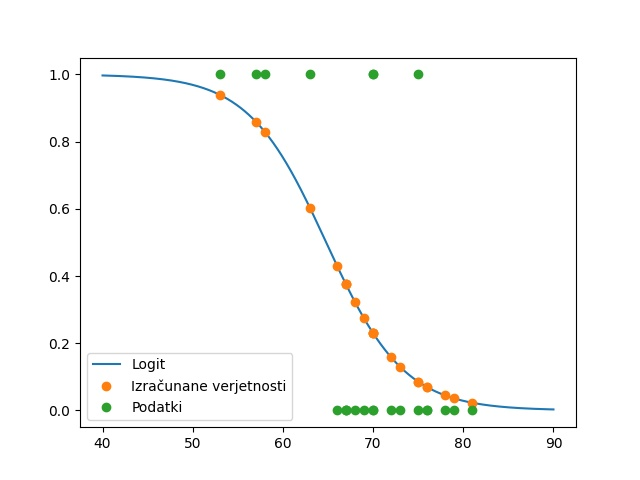
\includegraphics[scale=0.6]{logit_challenger.jpeg}
%\end{figure}
%
%\end{frame}

%\begin{frame}{Kaj še bom naredil}
%    \begin{itemize}
%        \item Analiziral časovno zahtevnost že postavljenega algoritma
%        \item Izvedel podobno še za kak drugačen model
%        \item Teorijo razvil še za splošen posplošen linearen model
%    \end{itemize}
%\end{frame}

\begin{frame}[t,allowframebreaks]
    \frametitle{References}
    \nocite{*}
    \printbibliography
\end{frame}
\end{document}